% \begin{figure}
%   \centering
%   \begin{tikzpicture}    
%     \node at (10, 0) {
%       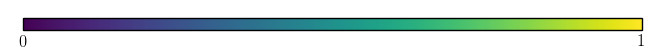
\includegraphics[height=4.2cm]{experiments/3d/vae_occ/easy_15/colorbar}
%     };
    
%     \node at (0, 0){
%       \includegraphics[width=6cm]{experiments/shapenet/vae_occ_aml/moderate_15_long_5/results_0}
%     };
    
%     \node at (6.5, 0){
%       \includegraphics[width=6cm]{experiments/shapenet/vae_occ_aml/moderate_15_long_5/results_3}
%     };
    
%     \draw[-,dashed](-3.5,-2.15) -- (10,-2.15);
    
%     % --- 
%     \node at (0, -3.5){
%       \includegraphics[width=6cm]{experiments/shapenet/baseline/moderate_15/results_0}
%     };
    
%     \node at (6.5, -3.5){
%       \includegraphics[width=6cm]{experiments/shapenet/baseline/moderate_15/results_3}
%     };
    
%     \node[rotate=90] at (-3.5, -3.5) {Baseline};
%     \node[rotate=90] at (-3.5, 0) {\AML};
%     %\node at (3.25, 2.5) {reconstruction};
%   \end{tikzpicture}
%   \vskip 6px
  
%   % TODO short caption
%   \caption{Qualitative results comparing \AML with the supervised baseline on the
%   \moderate case of our ShapeNet dataset. For \AML we show the observed points,
%   the partial free space, the ground truth shape and the predicted shape
%   including its error. We consider occupancy only. For the baseline, we merely
%   show the target shape, the predicted shape as well as its error. For both,
%   we show two samples. In the case of \AML, we can also see the uncertainty
%   of the predicted shapes, \eg along the wheels and the roof
%   in the second example on the right.}
%   \label{fig:appendix-experiments-shapenet-aml-qual-1}
% \end{figure}
\begin{figure}
  \hspace*{-0.5cm}
  \begin{tikzpicture}
    \node at (0, 0) {
      \includegraphics[width=3.75cm,trim={3.5cm 2.5cm 3.5cm 2.5cm},clip]{experiments/shapenet/vae_occ_aml/hard_15_long_statistics_75/1_input_45}
    };
    \node at (3.5, 0) {
      \includegraphics[width=3.75cm,trim={3.5cm 2.5cm 3.5cm 2.5cm},clip]{experiments/shapenet/vae_occ_aml/hard_15_long_statistics_75/1_prediction_45}
    };
    \node at (7, 0) {
      \includegraphics[width=3.75cm,trim={3.5cm 2.5cm 3.5cm 2.5cm},clip]{experiments/shapenet/vae_occ_aml/hard_15_long_statistics_75/1_target_45}
    };
    \node at (10.5, 0) {
      \includegraphics[width=3.75cm,trim={3.5cm 2.5cm 3.5cm 2.5cm},clip]{experiments/shapenet/baseline/hard_15/1_prediction_45}
    };
    
    \node at (0, -3) {
      \includegraphics[width=3.75cm,trim={3.5cm 2.5cm 3.5cm 2.5cm},clip]{experiments/shapenet/vae_occ_aml/hard_15_long_statistics_75/2_input_45}
    };
    \node at (3.5, -3) {
      \includegraphics[width=3.75cm,trim={3.5cm 2.5cm 3.5cm 2.5cm},clip]{experiments/shapenet/vae_occ_aml/hard_15_long_statistics_75/2_prediction_45}
    };
    \node at (7, -3) {
      \includegraphics[width=3.75cm,trim={3.5cm 2.5cm 3.5cm 2.5cm},clip]{experiments/shapenet/vae_occ_aml/hard_15_long_statistics_75/2_target_45}
    };
    \node at (10.5, -3) {
      \includegraphics[width=3.75cm,trim={3.5cm 2.5cm 3.5cm 2.5cm},clip]{experiments/shapenet/baseline/hard_15/2_prediction_45}
    };

    \draw[-,dashed] (-1.5,-4.75) -- (12,-4.75);

    \node at (0, -6.5) {
      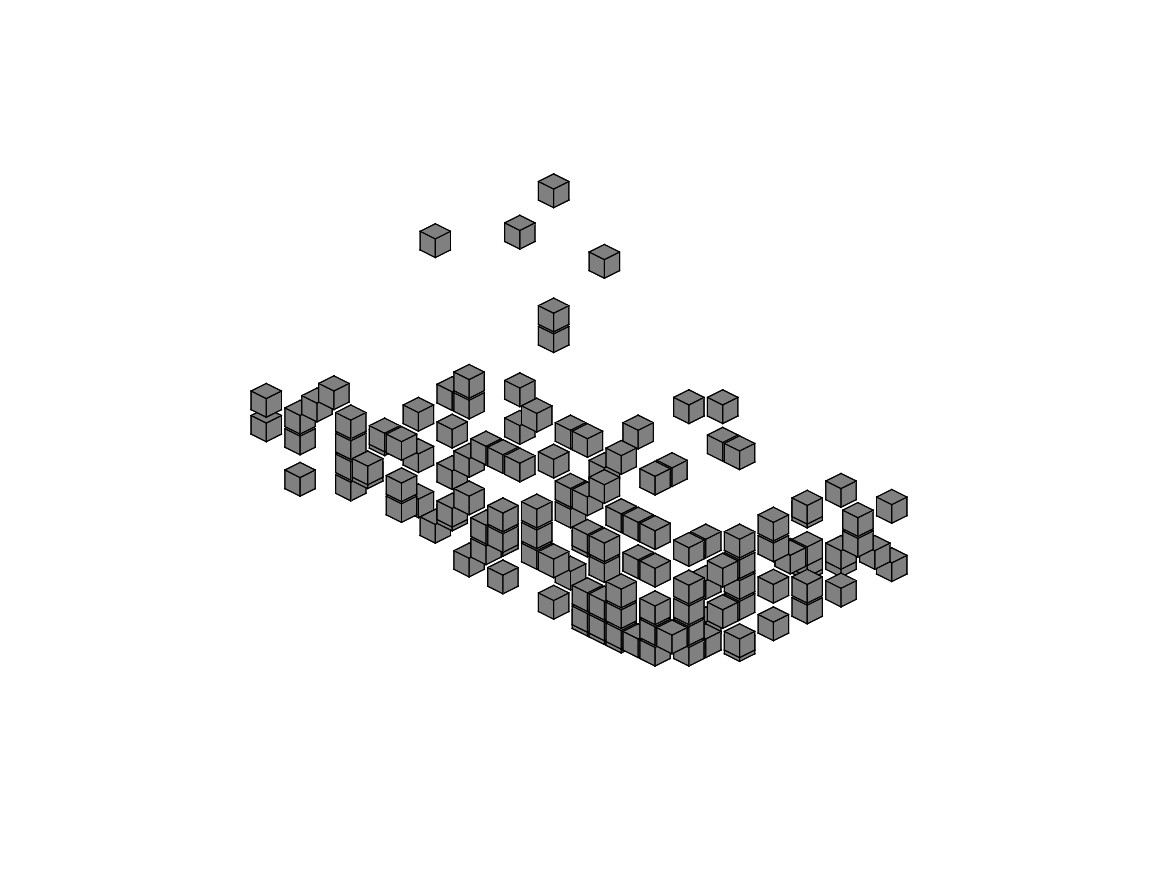
\includegraphics[width=3.75cm,trim={3.5cm 2.5cm 3.5cm 2.5cm},clip]{experiments/shapenet/vae_occ_aml/moderate_15_long_5/0_input_45}
    };
    \node at (3.5, -6.5) {
      \includegraphics[width=3.75cm,trim={3.5cm 2.5cm 3.5cm 2.5cm},clip]{experiments/shapenet/vae_occ_aml/moderate_15_long_5/0_prediction_45}
    };
    \node at (7, -6.5) {
      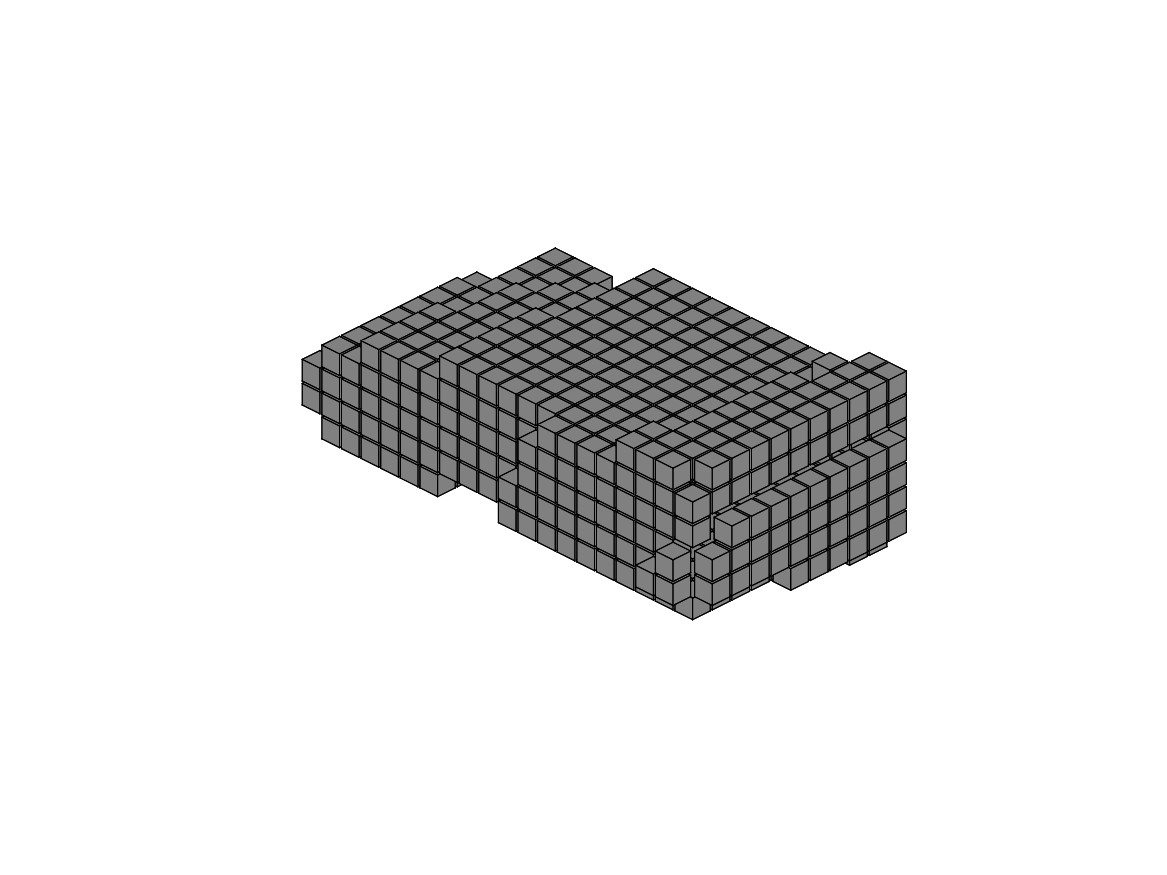
\includegraphics[width=3.75cm,trim={3.5cm 2.5cm 3.5cm 2.5cm},clip]{experiments/shapenet/vae_occ_aml/moderate_15_long_5/0_target_45}
    };
    \node at (10.5, -6.5) {
      \includegraphics[width=3.75cm,trim={3.5cm 2.5cm 3.5cm 2.5cm},clip]{experiments/shapenet/baseline/moderate_15/0_prediction_45}
    };
    
    \node at (0, -9.5) {
      \includegraphics[width=3.75cm,trim={3.5cm 2.5cm 3.5cm 2.5cm},clip]{experiments/shapenet/vae_occ_aml/moderate_15_long_5/1_input_45}
    };
    \node at (3.5, -9.5) {
      \includegraphics[width=3.75cm,trim={3.5cm 2.5cm 3.5cm 2.5cm},clip]{experiments/shapenet/vae_occ_aml/moderate_15_long_5/1_prediction_45}
    };
    \node at (7, -9.5) {
      \includegraphics[width=3.75cm,trim={3.5cm 2.5cm 3.5cm 2.5cm},clip]{experiments/shapenet/vae_occ_aml/moderate_15_long_5/1_target_45}
    };
    \node at (10.5, -9.5) {
      \includegraphics[width=3.75cm,trim={3.5cm 2.5cm 3.5cm 2.5cm},clip]{experiments/shapenet/baseline/moderate_15/1_prediction_45}
    };
    
    \node at (0, -12.5) {
      \includegraphics[width=3.75cm,trim={3.5cm 2.5cm 3.5cm 2.5cm},clip]{experiments/shapenet/vae_occ_aml/moderate_15_long_5/2_input_45}
    };
    \node at (3.5, -12.5) {
      \includegraphics[width=3.75cm,trim={3.5cm 2.5cm 3.5cm 2.5cm},clip]{experiments/shapenet/vae_occ_aml/moderate_15_long_5/2_prediction_45}
    };
    \node at (7, -12.5) {
      \includegraphics[width=3.75cm,trim={3.5cm 2.5cm 3.5cm 2.5cm},clip]{experiments/shapenet/vae_occ_aml/moderate_15_long_5/2_target_45}
    };
    \node at (10.5, -12.5) {
      \includegraphics[width=3.75cm,trim={3.5cm 2.5cm 3.5cm 2.5cm},clip]{experiments/shapenet/baseline/moderate_15/2_prediction_45}
    };
    
    \node at (0, -15.5) {
      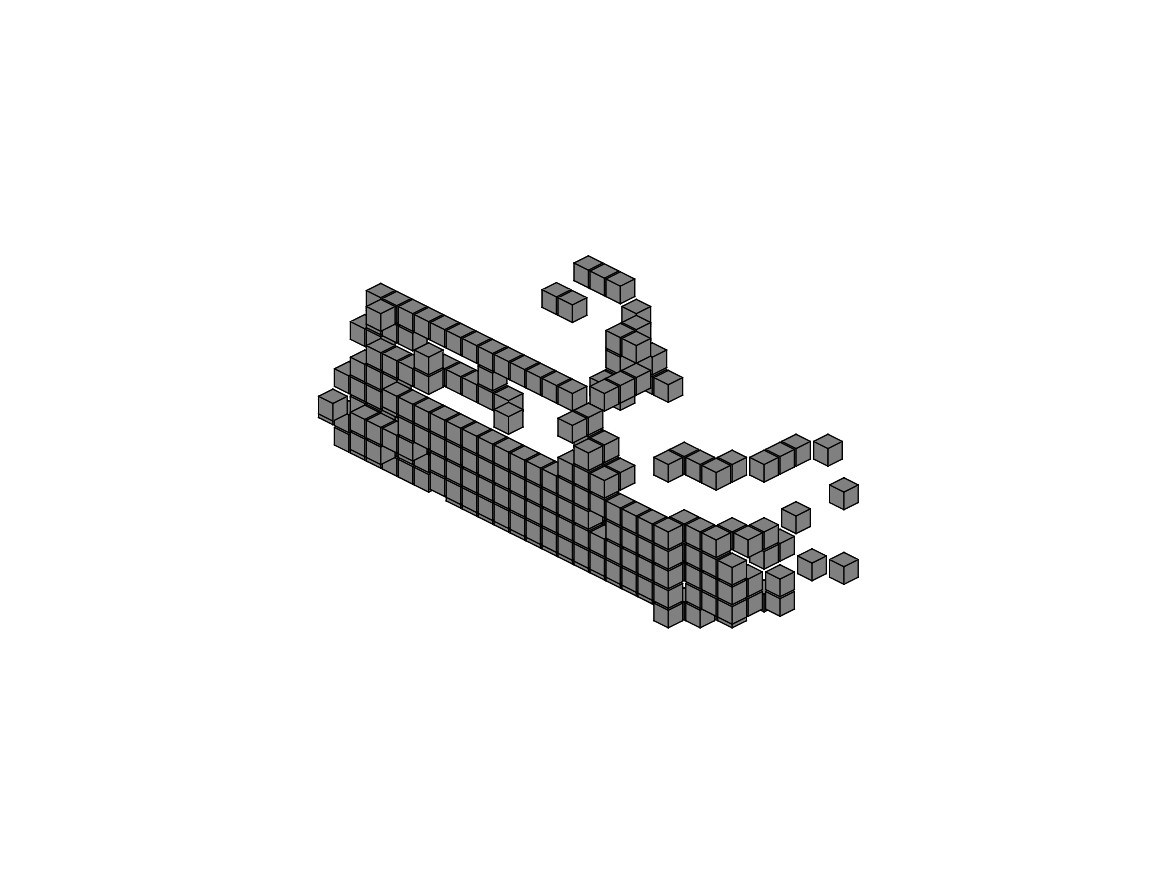
\includegraphics[width=3.75cm,trim={3.5cm 2.5cm 3.5cm 2.5cm},clip]{experiments/shapenet/vae_occ_aml/moderate_15_long_5/3_input_45}
    };
    \node at (3.5, -15.5) {
      \includegraphics[width=3.75cm,trim={3.5cm 2.5cm 3.5cm 2.5cm},clip]{experiments/shapenet/vae_occ_aml/moderate_15_long_5/3_prediction_45}
    };
    \node at (7, -15.5) {
      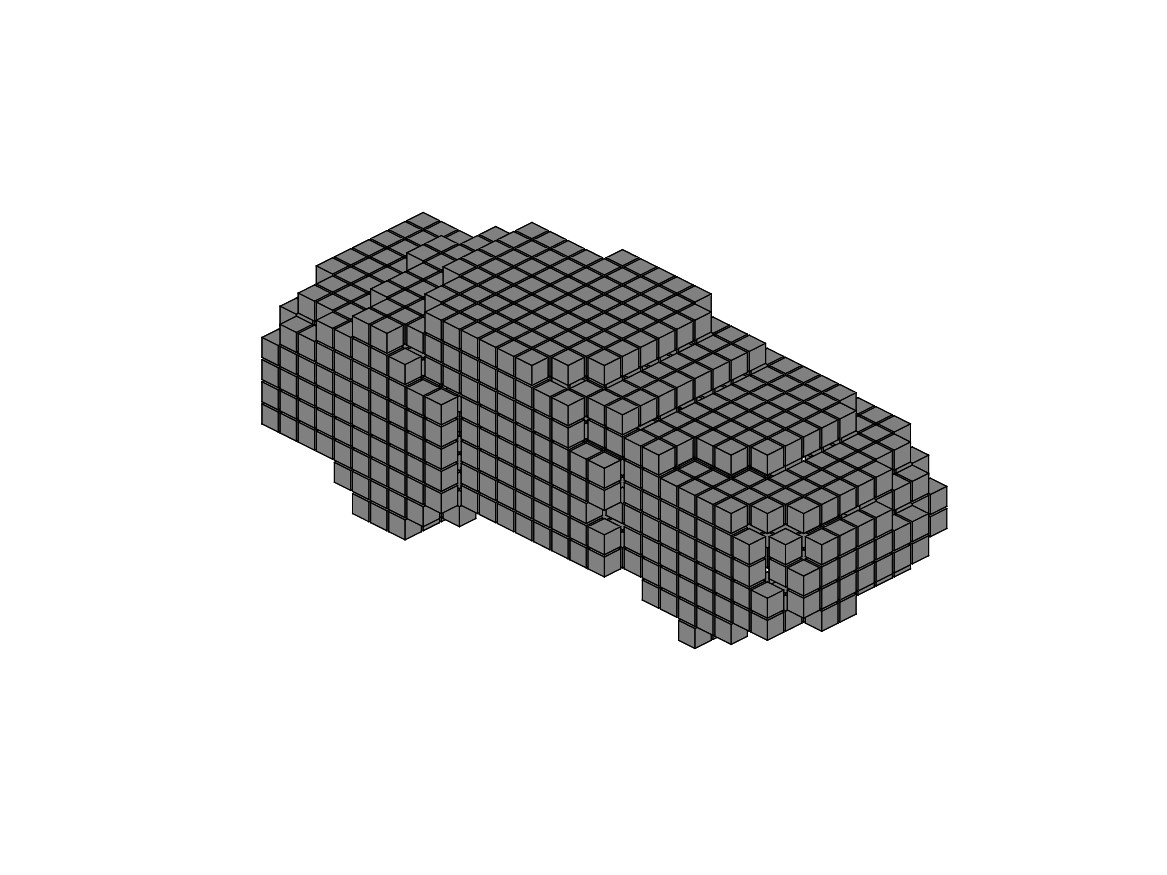
\includegraphics[width=3.75cm,trim={3.5cm 2.5cm 3.5cm 2.5cm},clip]{experiments/shapenet/vae_occ_aml/moderate_15_long_5/3_target_45}
    };
    \node at (10.5, -15.5) {
      \includegraphics[width=3.75cm,trim={3.5cm 2.5cm 3.5cm 2.5cm},clip]{experiments/shapenet/baseline/moderate_15/3_prediction_45}
    };

    \node[rotate=90] at (-2.5, -11) {\moderate};
    \node[rotate=90] at (-2.5, -1.5) {\hard};

    \node at (0, 1.75) {Input};
    \node at (3.5, 1.75) {\AML};
    \node at (7, 1.75) {Baseline};
    \node at (10.5, 1.75) {Target};
  \end{tikzpicture}
  \caption{Qualitative results for \AML and the supervised baseline for the \moderate and \hard
  cases of our ShapeNet-based dataset. We show the occupancy grids corresponding to
  the observed points, the \AML prediction, the prediction from the supervised baseline
  and the target shape.}
  \label{fig:appendix-experiments-shapenet-aml-qual-2}
\end{figure}
% \begin{figure}
%   \begin{tikzpicture}    
%     \node at (-3.5,0) {
%       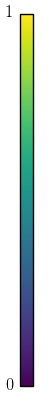
\includegraphics[height=4.25cm]{experiments/3d/vae_occ_sdf/colorbar_0}
%     };
    
%     \node at (0, 0){
%       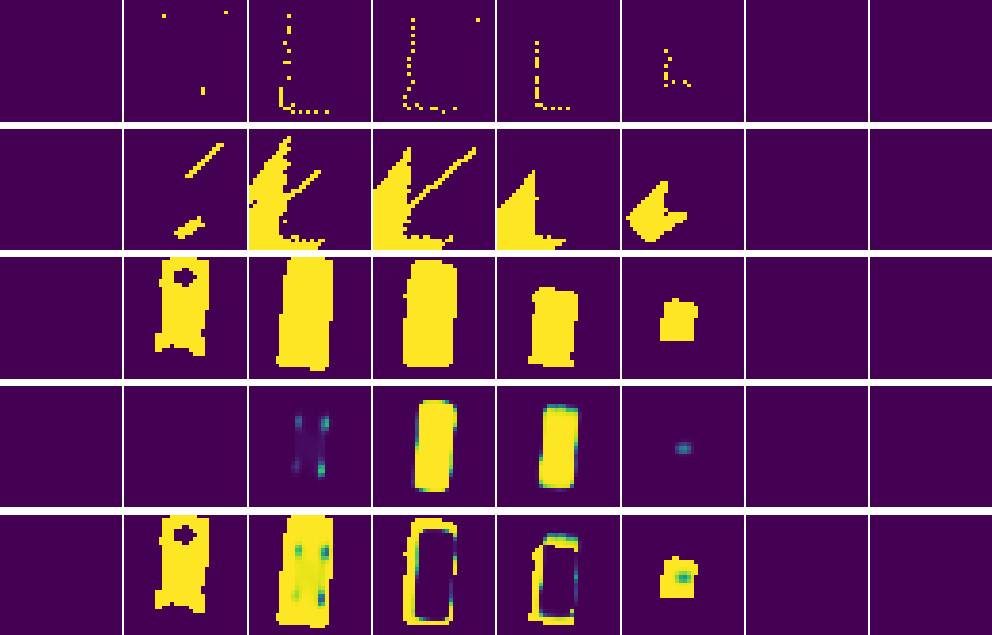
\includegraphics[width=6cm]{experiments/shapenet/vae_occ_sdf_aml/moderate_15/results_0_0}
%     };
%     \node at (0, -4){
%       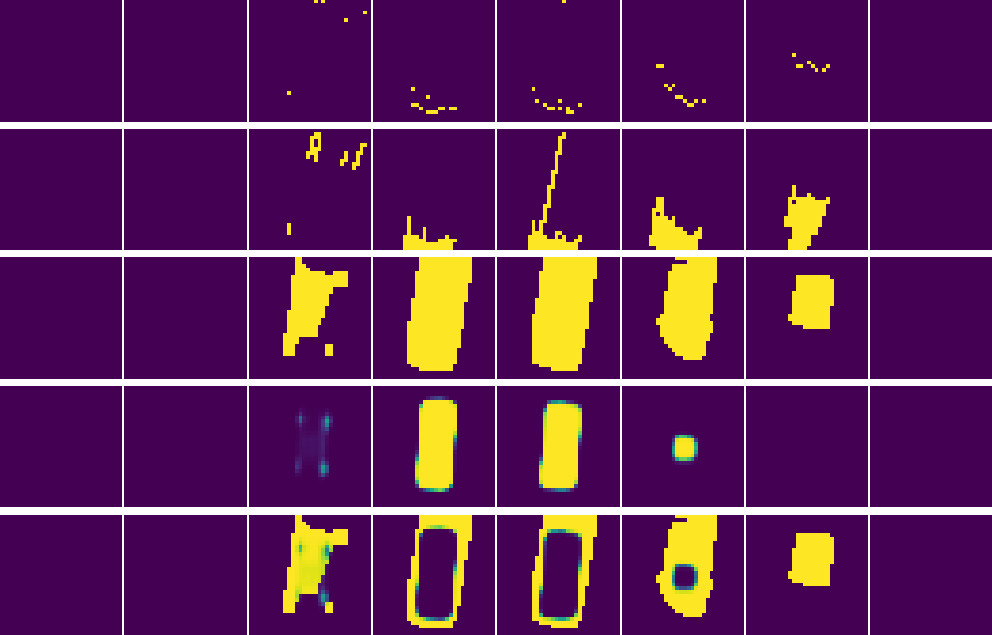
\includegraphics[width=6cm]{experiments/shapenet/vae_occ_sdf_aml/moderate_15/results_3_0}
%     };
    
%     \node at (6.5, 0){
%       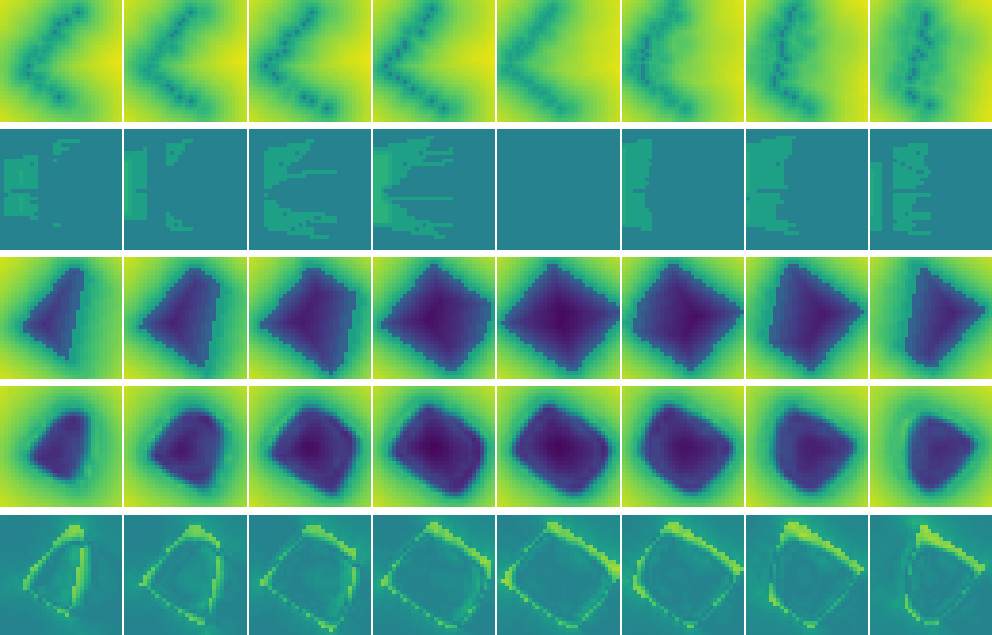
\includegraphics[width=6cm]{experiments/shapenet/vae_occ_sdf_aml/moderate_15/results_0_1}
%     };
%     \node at (6.5, -4){
%       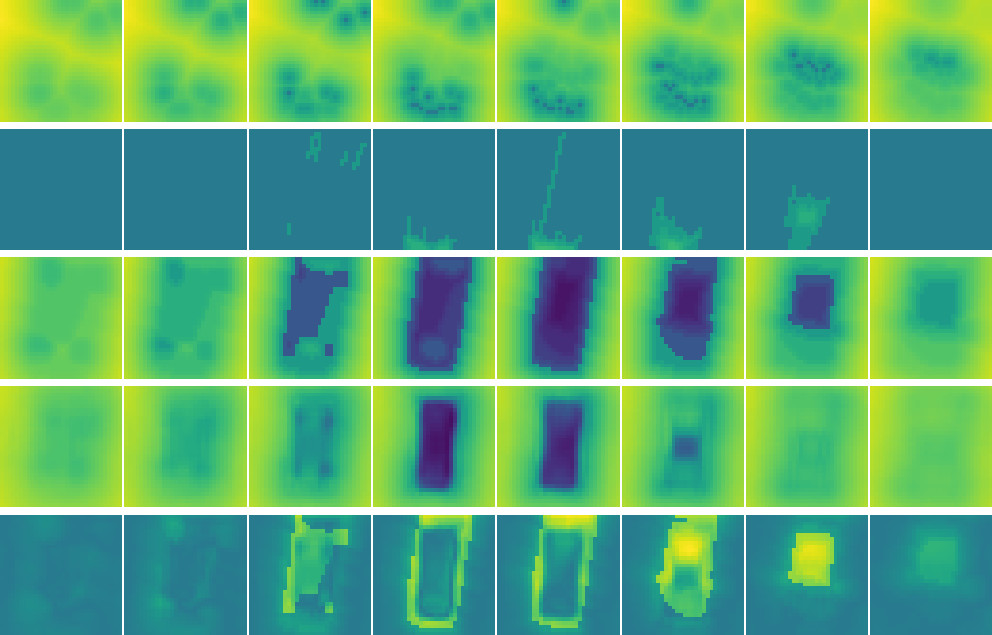
\includegraphics[width=6cm]{experiments/shapenet/vae_occ_sdf_aml/moderate_15/results_3_1}
%     };
    
%     \node at (10,0) {
%       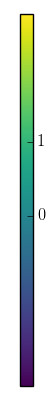
\includegraphics[height=4.25cm]{experiments/3d/vae_occ_sdf/colorbar_1}
%     };
    
%     \node at (0, 2.25) {occupancy};
%     \node at (6.5, 2.25) {signed distance function};
%   \end{tikzpicture}
%   \vskip 6px

%   % TODO short caption
%   \caption{Qualitative results for \AML on moderate difficulty using both
%   occupancy and signed distance functions for shape representation. We show
%   both modalities for two examples, including the observed points, the 
%   partial free space, the target shape and the predicted shape with its error.
%   In all cases we show horizontal slices of the corresponding volumes,
%   in particular heights $8 + 2i$ for $0 \leq i < 7$. Compared to Figure
%   \ref{fig:appendix-experiments-shapenet-aml-qual-1}, the predicted shapes
%   look slightly worse. In the second case, the target shape is also underestimated
%   in size which we also observed in the \hard case. 3D visualizations can be found
%   in Figure \ref{fig:appendix-experiments-shapenet-aml-qual-4}.}
%   \label{fig:appendix-experiments-shapenet-aml-qual-3}
% \end{figure}
\begin{figure}[t]
  \centering
  \begin{tikzpicture}

    \node at (0, 0) {
      \includegraphics[width=2.75cm,trim={1cm 2cm 1cm 2cm},clip]{experiments/shapenet/vae_occ_sdf_aml/hard_15_statistics/0_prediction}
    };
    \node at (3, 0) {
      \includegraphics[width=2.75cm,trim={1cm 2cm 1cm 2cm},clip]{experiments/shapenet/vae_occ_sdf_aml/hard_15_statistics/0_target}
    };
    
    \node at (7, 0) {
      \includegraphics[width=2.75cm,trim={1cm 2cm 1cm 2cm},clip]{experiments/shapenet/vae_occ_sdf_aml/hard_15_statistics/3_prediction}
    };
    \node at (10, 0) {
      \includegraphics[width=2.75cm,trim={1cm 2cm 1cm 2cm},clip]{experiments/shapenet/vae_occ_sdf_aml/hard_15_statistics/3_target}
    };

    \draw[-,dashed] (-1.5,-1.25) -- (11.5,-1.25);

    \node at (0, -2.5) {
      \includegraphics[width=2.75cm,trim={1cm 2cm 1cm 2cm},clip]{experiments/shapenet/vae_occ_sdf_aml/moderate_15/0_prediction}
    };
    \node at (3, -2.5) {
      \includegraphics[width=2.75cm,trim={1cm 2cm 1cm 2cm},clip]{experiments/shapenet/vae_occ_sdf_aml/moderate_15/0_target}
    };
    
    \node at (7, -2.5) {
      \includegraphics[width=2.75cm,trim={1cm 2cm 1cm 2cm},clip]{experiments/shapenet/vae_occ_sdf_aml/moderate_15/3_prediction}
    };
    \node at (10, -2.5) {
      \includegraphics[width=2.75cm,trim={1cm 2cm 1cm 2cm},clip]{experiments/shapenet/vae_occ_sdf_aml/moderate_15/3_target}
    };
    
    \node at (0, -4.5) {
      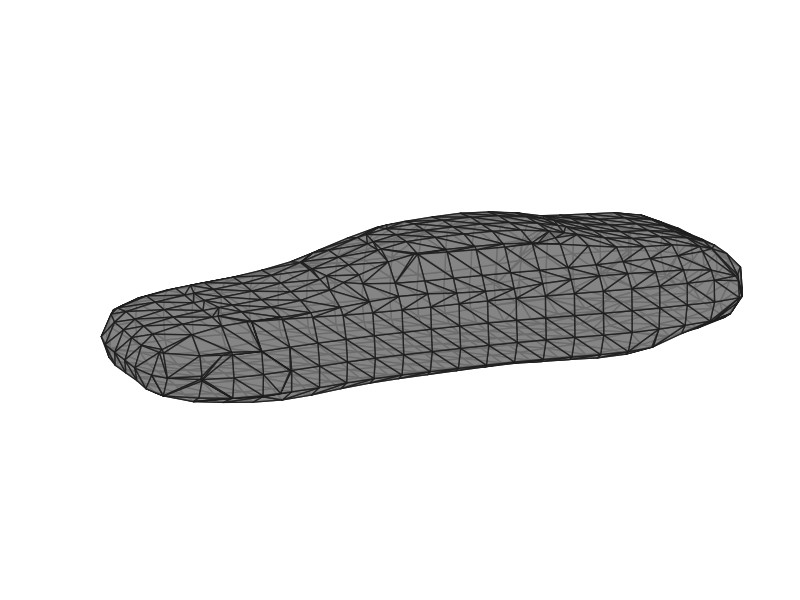
\includegraphics[width=2.75cm,trim={1cm 2cm 1cm 2cm},clip]{experiments/shapenet/vae_occ_sdf_aml/moderate_15/1_prediction}
    };
    \node at (3, -4.5) {
      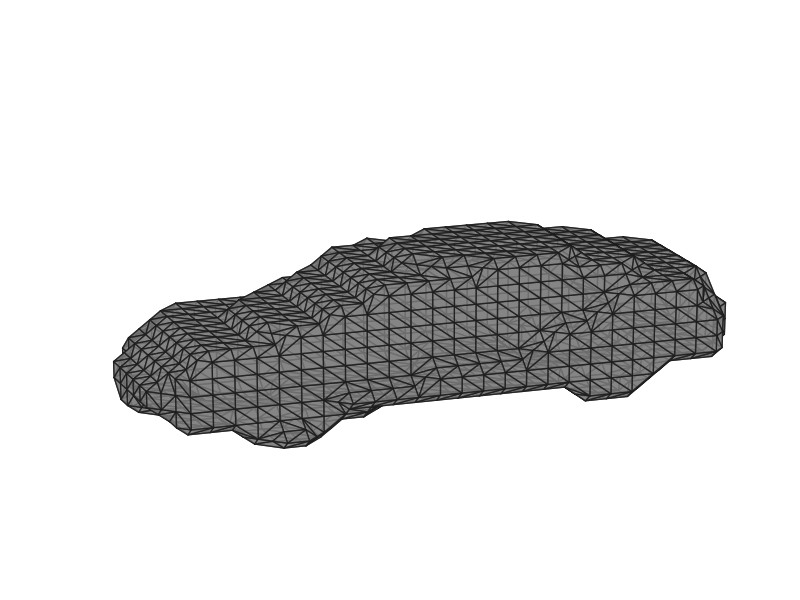
\includegraphics[width=2.75cm,trim={1cm 2cm 1cm 2cm},clip]{experiments/shapenet/vae_occ_sdf_aml/moderate_15/1_target}
    };
    
    \node at (7, -4.5) {
      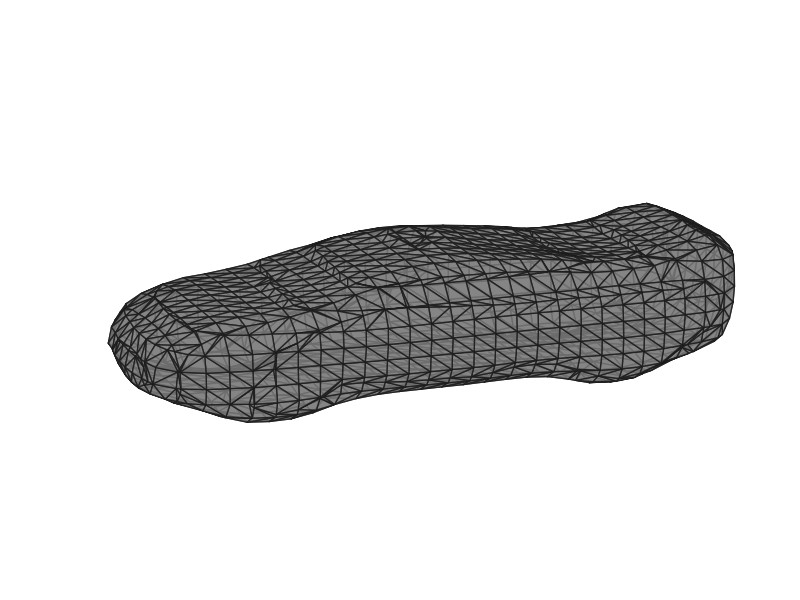
\includegraphics[width=2.75cm,trim={1cm 2cm 1cm 2cm},clip]{experiments/shapenet/vae_occ_sdf_aml/moderate_15/2_prediction}
    };
    \node at (10, -4.5) {
      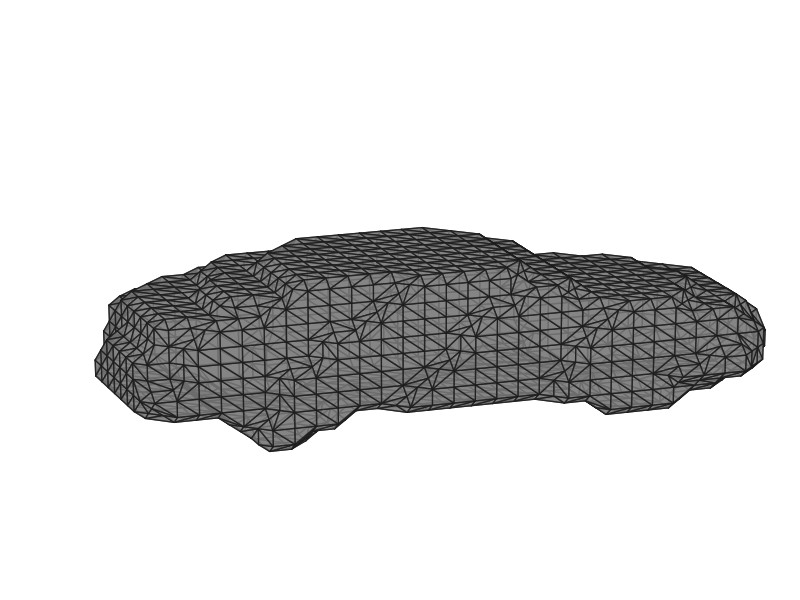
\includegraphics[width=2.75cm,trim={1cm 2cm 1cm 2cm},clip]{experiments/shapenet/vae_occ_sdf_aml/moderate_15/2_target}
    };

    \draw[-,dashed] (5,-5.5) -- (5, 1);

    \node[rotate=90] at (-2.5, 0) {\hard};
    \node[rotate=90] at (-2.5, -3.5) {\moderate};

    \node at (0, 1) {\AML};
    \node at (3, 1) {Target};
    \node at (7, 1) {\AML};
    \node at (10, 1) {Target};
  \end{tikzpicture}
  \caption{3D visualizations of \AML using both occupancy and signed distance functions
  on the ShapeNet dataset.
  Here we show meshes obtained from marching cubes applied on the predicted
  signed distance functions in comparison to the corresponding targets. We note that
  the signed distance functions are derived from the corresponding occupancy grids;
  this explains the ``voxelized'' appearance of the ground truth meshes.}
  \label{fig:appendix-experiments-shapenet-aml-qual-4}
\end{figure}
